\documentclass[18pt]{article}
\usepackage{graphicx}
\usepackage{amsmath}
\graphicspath{{./images/}}
\usepackage{subcaption}

\title{Neural Network and Deep Learning, \\ Micahel Nielsen, Chapter 1}
\author{Utkarsh Tiwari}

\begin{document}

\maketitle

\textbf{Sigmoid neurons simulating perceptrons, part I} \\
Question 1: Suppose we take all the weights and biases in a network of perceptrons, and multiply them by a positive constant, $c>0$
. Show that the behaviour of the network doesn't change. \\ \\
Solution: for perceptrons: $$
output=f(w,x,b)=
\begin{cases}
0 & \text{if } w\cdot x+b \leq 0 \\
1 & \text{if } w\cdot x+b > 0
\end{cases}
$$ 
where $b \equiv -\text{threshold}$,
$w \cdot x \equiv \sum_{j} w_j x_j, \text{ where } w \text{ and } x \text{ are weight and input vectors respectively.}$
\\
After multiplying with a positive constant $c>0$: $$
output=f(w,x,b)=
\begin{cases}
0 & \text{if } cw\cdot x+cb \leq 0 \\
1 & \text{if } cw\cdot x+cb > 0
\end{cases}
$$
$$
=output=f(w,x,b)=
\begin{cases}
0 & \text{if } c(w\cdot x+b) \leq 0 \\
1 & \text{if } c(w\cdot x+b) > 0
\end{cases}
$$
$$
=output=f(w,x,b)=
\begin{cases}
0 & \text{if } (w\cdot x+b) \leq 0 \\
1 & \text{if } (w\cdot x+b) > 0
\end{cases}
$$

\textbf{Q.E.D}

\\
\textbf{Sigmoid neurons simulating perceptrons, part II} \\

Question 2: Suppose we have the same setup as the last problem - a network of perceptrons. Suppose also that the overall input to the network of perceptrons has been chosen. We won't need the actual input value, we just need the input to have been fixed. Suppose the weights and biases are such that $w \cdot x + b \neq 0$
 for the input $x$ to any particular perceptron in the network. Now replace all the perceptrons in the network by sigmoid neurons, and multiply the weights and biases by a positive constant $c>0$
. Show that in the limit as $c \rightarrow \infty$
 the behaviour of this network of sigmoid neurons is exactly the same as the network of perceptrons. How can this fail when $w⋅x+b=0$
 for one of the perceptrons? \\ \\
Solution: For Sigmoid Neurons:
$$
output=f(w,x,b)= \sigma(-w\cdot x-b)
$$ 
where, $$
\sigma(z)=\frac{1}{1 + e^{-z}}
$$
\textbf{Assumption}:
Assume that $x$ is a fixed unknown value where $w \cdot x + b \neq 0$. Then the resulting network will remain unchanged (assuming $c > 0$) as $c \rightarrow \infty$.

\textbf{Case 1}:$$w \cdot x + b < 0:$$\\
$$output=\lim_{c \rightarrow \infty} \frac{1}{1 + e^{c(-w\cdot x-b)}}$$
$$\implies output=\frac{1}{1+e^(\lim_{c \rightarrow \infty}c(-w\cdot x-b)}$$
$$=\frac{1}{1+e^\inf}$$
$$=0$$

\textbf{Case 2}:$$w \cdot x + b > 0:$$\\
$$output=\lim_{c \rightarrow \infty} \frac{1}{1 + e^{c(-w\cdot x-b)}}$$
$$\implies output=\frac{1}{1+e^(\lim_{c \rightarrow \infty}c(-w\cdot x-b)}$$
$$=\frac{1}{1+e^-(\inf)}$$
$$=1$$

This is exactly like a perceptron. \textbf{Q.E.D}

\textbf{Case 3}:$$w \cdot x + b = 0:$$\\
$$output=\lim_{c \rightarrow \infty} \frac{1}{1 + e^{c(-w\cdot x-b)}}$$
$$\implies output=\frac{1}{1+e^(\lim_{c \rightarrow \infty}c(0))}$$
$$=\frac{1}{1+e^0}$$
$$=1/2$$

\textbf{Alternate Approach:}
The sigmoid function (activation function for sigmoid neuron) is a smoothed version of the step function (activation function for perceptron)
\begin{figure}[htbp]
  \centering
  \begin{subfigure}[b]{0.4\textwidth}
    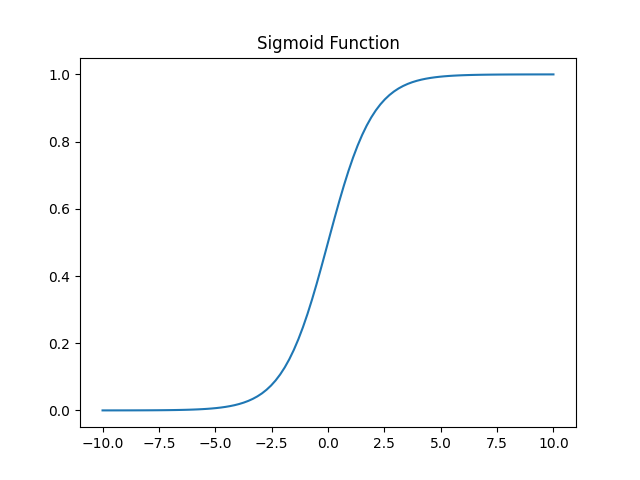
\includegraphics[width=1.3\textwidth]{images/sigmoid.png}
    \caption{Sigmoid Function}
    \label{fig:sigmoid}
  \end{subfigure}
  \hspace{1cm}
  \begin{subfigure}[b]{0.4\textwidth}
    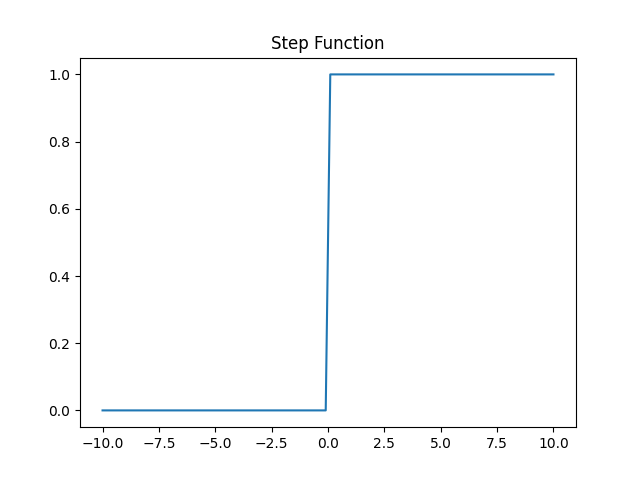
\includegraphics[width=1.3\textwidth]{images/step.png}
    \caption{Step Function}
    \label{fig:step}
  \end{subfigure}
\end{figure}

If the input(s) of the sigmoid function is multiplied by a positive constant $c$ where $c\rightarrow \infty$ then the plot of the sigmoid function starts approaching the shape of the step function.


\begin{figure}[htbp]
    \centering
    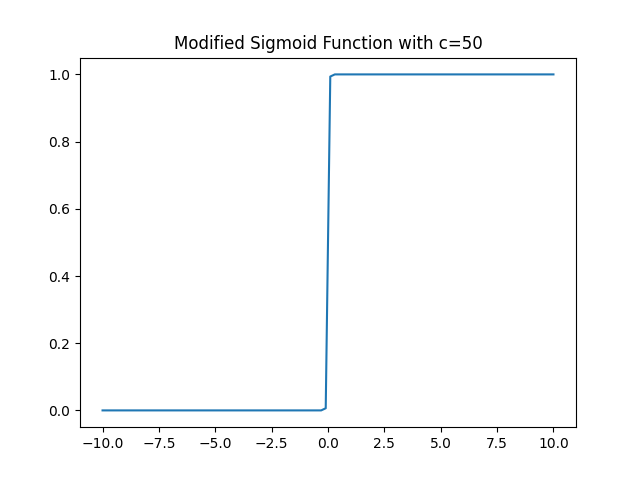
\includegraphics[width=0.7\textwidth]{images/Figure_4.png}
    \caption{Sigmoid Function with c=50 starts resembling the step function. The modified function is $\frac{1}{1+e^(cz)}$}
    \label{fig:my_label}
\end{figure}

So, we can see that as $c \rightarrow \infty$ the activation function on the sigmoid neurons starts resembling the step function. Hence, there is no difference between the two under the given condition. \textbf{Q.E.D}\\
Also, because the step function is undefined for $x=0$ we cannot comment whether the above proved statement holds when $w\cdot x + b = 0$.


\end{document}